
%(BEGIN_QUESTION)
% Copyright 2007, Tony R. Kuphaldt, released under the Creative Commons Attribution License (v 1.0)
% This means you may do almost anything with this work of mine, so long as you give me proper credit

Shown here is a pair of loop-powered 4-20 mA process transmitters, a process controller with dual measurement inputs, and a 4-20 mA I/P (current-to-pressure) converter used to drive a pneumatically-actuated control valve.  The controller inputs are ranged from 1 to 5 volts DC, not 4-20 mA:

$$\includegraphics[width=15.5cm]{i02273x01.eps}$$
Show how all three field devices would properly connect to the controller, including the placement of resistors to convert the current signals into voltage signals that the controller's ADC's may interpret.  Furthermore, use shielded cable, showing where all shield ground connections should be located.

\vfil 

\underbar{file i02273}
\eject
%(END_QUESTION)





%(BEGIN_ANSWER)

This is a graded question -- no answers or hints given!

%(END_ANSWER)





%(BEGIN_NOTES)

A helpful problem-solving tip when sketching wires for any DC circuit is to identify all {\it sources} and {\it loads}, then sketch arrows showing the appropriate directions of current based on the device voltage polarity:

$$\includegraphics[width=15.5cm]{i02273x02.eps}$$

%INDEX% Basics, 2-wire loop-powered transmitter: connection to process controller

%(END_NOTES)


